\documentclass[11pt,fleqn]{article}

\usepackage{amsmath}
\usepackage{amssymb}
\usepackage{url}
\usepackage{listings}
\usepackage{color}
\usepackage{tikz}
\usetikzlibrary{automata,positioning,arrows}
\usepackage{diagbox}
%\usepackage[normalem]{ulem}

\lstset{language=python,basicstyle=\ttfamily,breaklines=true,showspaces=false,showstringspaces=false,breakatwhitespace=true,texcl=true,escapeinside={\%*}{*)}}

\setlength {\topmargin} {-.15in}
\setlength {\textheight} {8.6in}

\input{../def}

\begin{document}

\bc

  {\large \textbf{COMPSCI/SFWRENG 2FA3}}\\[2mm]
  {\large \textbf{Discrete Mathematics with Applications II}}\\[2mm]
  {\large \textbf{Winter 2020}}\\[8mm]
  {\huge \textbf{Week 08 Exercises}}\\[6mm]
  {\large \textbf{Dr.~William M. Farmer}}\\[2mm]
  {\large \textbf{McMaster University}}\\[6mm]
  {\large Revised: February 24, 2020}

\ec

\medskip

\subsection*{Exercises}

\be

  \item Construct a NFA $N = (Q,\Sigma,\Delta,S,F)$ such that $\Sigma
    = \set{0,1}$ and $L(N)$ is the set of strings in $\Sigma^*$ that
    contain two consecutive 0s or two consecutive 1s.

  \item Consider the following NFA $N$ over $\set{a,b}$ defined by the
    following transition diagram:

\bc
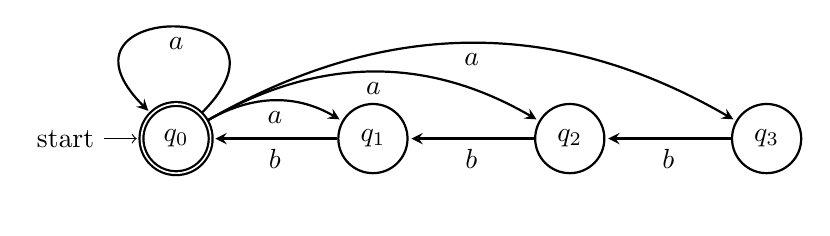
\begin{tikzpicture}[shorten >=1pt,node distance=2.5cm,on grid,auto] 
   \node[state, initial, accepting, thick] (q_0)   {$q_0$}; 
   \node[state, thick] (q_1) [right=of q_0] {$q_1$}; 
   \node[state, thick] (q_2) [right=of q_1] {$q_2$}; 
   \node[state, thick] (q_3) [right=of q_2] {$q_3$};
    \path[->, thick, >=stealth] 
    (q_0) edge [loop, below] node {$a$} (q_0)
          edge [bend left, below] node {$a$} (q_1)
          edge [bend left, below] node {$a$} (q_2)
          edge [bend left, below] node {$a$} (q_3)
    (q_1) edge [right, below] node {$b$} (q_0)
    (q_2) edge [right, below] node {$b$} (q_1) 
    (q_3) edge [right, below] node {$b$} (q_2); 
\end{tikzpicture}
\ec

  \be

    \item What is $L(N)$?

    \item Construct a DFA $M$ equivalent to $N$ that has no
      inaccessible states.

  \ee

  \item Construct an NFA $N$ for the alphabet $\Sigma = \set{a,b}$
    such that $L(N)$ is the set of all strings $x \in \Sigma^*$ in
    which at least one of the last three symbols of $x$ is an $a$ if
    $|x| \ge 3$ and at least one of the symbols of $x$ is an $a$ if
    $|x| < 3$.  Present $N$ as a transition diagram.

  \item Consider the NFA $N = (Q,\Sigma,\Delta,S,F)$ defined by the
    following transition table:

\bc
\begin{tabular}{r|l|ll|}
\cline{2-4}
& {\diagbox{$Q$}{$\Sigma$}} & $0$ & $1$\\
\cline{2-4}
start $\tarrow$ & $p$ & $\set{p,q}$ & $\set{p}$\\
                & $q$ & $\set{r}$   & $\set{r}$\\
                & $r$ & $\set{s}$    & $\set{}$\\
final $\tarrow$ & $s$ & $\set{s}$    & $\set{s}$\\
\cline{2-4}
\end{tabular}
\ec

    Construct a DFA $M$ equivalent to $N$ that has no inaccessible
    states.

  \item Let the \emph{reverse} of a string $x$, written,
    $\mname{rev}(x)$, be the string $x$ written backwards.  Also, for
    $A \subseteq \Sigma^*$, let $\mname{rev}(A) = \set{\mname{rev}(x)
    \mid x \in A}$.  Prove that, if $A \subseteq \Sigma^*$ is regular,
    then so is $\mname{rev}(A)$.

  \item\bsp Let $N = (Q_N,\Sigma,\Delta_N,S_N,F_N)$ be an NFA and $M =
    (Q_M,\Sigma,\delta_M,s_M,F_M)$ be obtained from $N$ by the subset
    construction.  Prove by induction on $|x|$,
    that \[\hat{\delta}_M(A,x) = \hat{\Delta}_N(A,x)\] for all $A
    \subseteq Q_N$ and $x \in \Sigma^*$.\esp

\ee
\end{document}


